\scanpage{15}\mspage{14}
En résumé, en termes de $\unsure{\mathcal{F}|\mathfrak{F}}$, c'est de la donnée de deux \uline{relations} \uline{d'ordre}
% The enclosure has no right side, and its left upright is separated from the top and bottom rules.
\figure{
\[
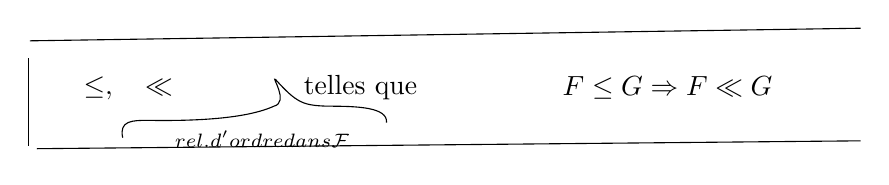
\begin{tikzpicture}[x=1cm,y=1cm,baseline=(orders.base)]
  \node (orders) at (1.25,0.10) {$\displaystyle \leq,\quad\ll$};
  \node at (4.20,0.10) {telles que};
  \node at (8.10,0.10) {$\displaystyle F\leq G\Rightarrow F\ll G$};
  \node at (2.95,-0.55) {$\scriptstyle\text{rel. d'ordre dans }\mathcal{F}$};
  \draw (1.18,-0.53) .. controls (1.13,-0.31) and (1.31,-0.31) .. (1.50,-0.31)
    .. controls (2.10,-0.32) and (2.75,-0.29) .. (3.10,-0.13)
    .. controls (3.30,-0.08) and (3.06,0.26) .. (3.12,0.21)
    .. controls (3.39,-0.09) and (3.47,-0.12) .. (3.78,-0.13)
    .. controls (4.15,-0.13) and (4.55,-0.14) .. (4.53,-0.34);
  \draw (0,0.70) -- (10.55,0.86);
  \draw (-0.02,0.48) -- (-0.02,-0.64);
  \draw (0.09,-0.67) -- (10.55,-0.57);
\end{tikzpicture}
\tag*{(1.30)}
\]
}
que je vais partir.

En termes de celles-ci, on definit \deleted{$\unsure{\mathcal{M}|M}$}
\[
\mathcal{M}\subset\mathcal{F}
\]
par (1.20), \unsure{avec} les relations $\underset{\mathcal{M}}{\leq},\ \underset{\mathcal{M}}{\ll}$ induites par $\underset{\mathcal{F}}{\leq},\ \underset{\mathcal{F}}{\ll}$, puis
\[
\mathcal{L}\subset\mathcal{M}
\]
par (1.25). L'application
\[
\mathcal{F}\hookrightarrow\unsure{\mathcal{P}|\mathscr{P}|\mathfrak{P}}(\mathcal{M})\qquad
\deleted{X}\inserted{F}\longmapsto\widetilde{F}=\mathrm{Dep}(F)
\tag*{($*$)}
\]
% At the first map source, the live F is superimposed on the canceled X.
est \inserted{alors} definie par
\[
\widetilde{F}=\{X\in\mathcal{M}\mid X\leq F\}
\tag*{(1.31)}
\]
et
\[
\mathcal{F}\hookrightarrow\mathrm{Fig}(\mathcal{M})\qquad
\unsure{F|\deleted{F}|\deleted{X}F}\longmapsto\mathrm{Fig}_{\mathcal{M}}(F)
\tag*{($**$)}
\]
% The second source has one long rising oblique stroke through the upper part of F.
% It can be an entry stroke, a cancellation, or a remnant of X overwritten by F.
par (1.4) :
\[
\mathrm{Fig}_{\mathcal{M}}(F)=\{\widetilde{X}\mid X\in\widetilde{F}\}\subset\mathcal{P}(\mathcal{M})
\tag*{\deleted{(1.32)}}
\]
avec
\[
\widetilde{X}=\{Y\in\mathcal{M}\mid Y\leq X\}\quad.
\]

Ainsi, $\mathcal{F}$ est interprété comme un ens. de parties dans $\mathcal{M}$ via ($*$), et $\leq$ \unsure{s'interprète|s'interprête} simplement par l'inclusion
\[
F\leq G\Longleftrightarrow\widetilde{F}\subset\widetilde{G}
\tag*{(1.32)}
\]
